\usepackage{graphicx}

\section{Manuel d'utilisation}

\subsection{Mode Console}
\vspace{1cm}
\paragraph{}Pour l'utilisation du mode console, l'utilisateur doit lancer dans le package test le TesteConsole. Puis En lançant le « TestConsole », on nous invite à faire un choix en appuyant soit sur « 1 » pour le mode aléatoire ou « 2 » pour le mode manuel. Ici, nous allons appuyer sur « 1 » pour exécuter le mode Console. Si c’est un choix aléatoire, cela initialisera les variables aléatoirement le nombre de lignes et le nombre de colonnes de la grille. Si c’est un choix manuel, le programme invite à l’utilisateur de choisir les dimensions proposées de la grille : soit d’un format 12x12, 16x16 ou 20x20 (de type « nombreLignesxnombreColonnes »). 

\begin{center}
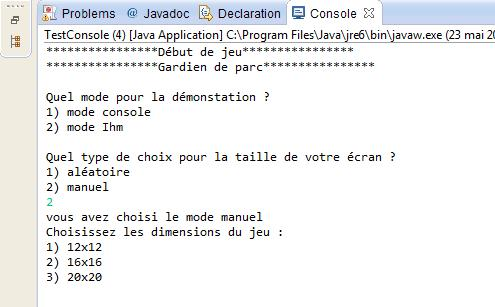
\includegraphics[height=200, width=400]{images/vu_consol.jpg}
\end{center}
\label{}Vue d'ensemble du mode console.
\vspace{1cm}
\paragraphe{}Ensuite, cela affichera la grille du jeu, ainsi que les éléments : Les gardiens sont représentés par G, S, C et P; les Intrus sont représentés par I, R et D; le reste par M(les murs), A(les arbres) et E(les eaux). 
Après avoir initialisé la grille, on passe en phase de test manuel des éléments du jeu. 
Par défaut, Si vous choisissez de saisir les touches différentes de « 5 » et « 6 », cela déplacera uniquement les Intrus (I, R et D). 
Si vous voulez déplacer l’un des gardiens (G, S, C et P), vous devez saisir la touche « 5 » pour sélectionner l’un d’eux. Une fois appuyé, vous devez choisir un chiffre entre 1 et 4 suivant les informations indiquées. Si vous saisissez la touche « 6 », on passera en phase de déplacement aléatoire où tous les gardiens et intrus bougeront sans cesse aléatoirement.

\begin{center}
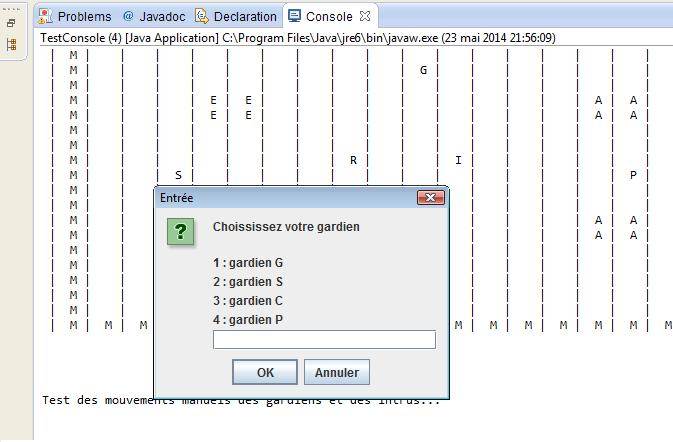
\includegraphics[height=200, width=500]{images/console.jpg}
\end{center}
\label{}Vue du mode 
\subsection{Mode graphique(IHM)}

\paragraph{}En lançant le « TestIhm », cela ouvrira un menu qui offrira deux options : Soit vous cliquez sur « Commencer » et vous lancez la partie ; soit vous cliquez sur « Quitter » et le programme sera fermé .Une fois le jeu lancé, on nous donne les règles du jeu. \\
Ensuite, cela affichera l’écran du jeu :
 
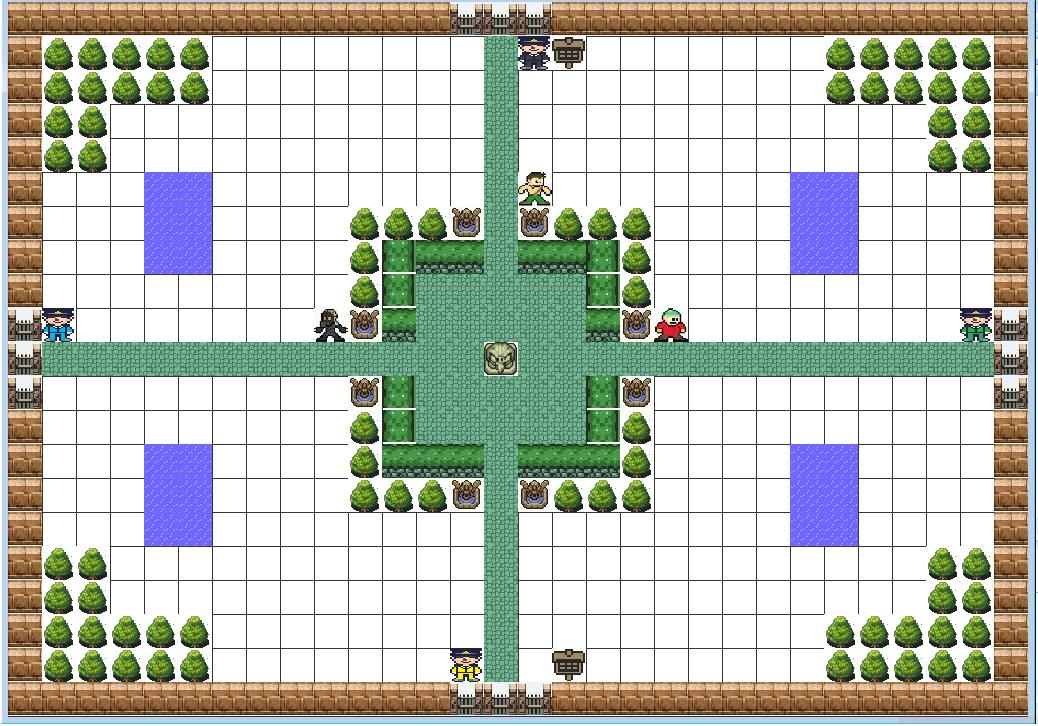
\includegraphics[height=200, width=500]{images/ihm.jpg}
%\figure{}Vue de l'IHM.


